\chapter{Soluciones de referencia}
\label{cap:capitulo6}

En este capítulo abordaremos la solución al problema Sigue Personas para los ejercicios \textit{Simulated Follow Person} y \textit{Real Follow Person} en este orden. Con los dos ejercicios el usuario podrá poner a prueba su algoritmo. Se pretende poner en práctica la experiencia del programador robótico cuando desarrolla una solución robótica. El primer paso es probar su programa en una simulación (\textit{Simulated Follow Person}), una vez que su solución es bastante robusta, pasa al siguiente nivel, probandolo en el mundo real (\textit{Real Follow Person}). El programador se dará cuenta de que es muy probable que el mismo programa en simulación no funcione igual que con un robot real. Entonces, si su solución era bastante buena, solamente tendrá que ajustar algunos parámetros y tener en cuenta ciertos factores (como el terreno) y habrá logrado su objetivo.\\

\section{Solución Sigue-Personas Simulado}
\label{sec:solucion_sigue_personas_simulado}

La solución que resuelve el problema de \textit{Seguir a una persona} lo podemos dividir en 3 subobjetivos: a) detección mediante Machine Learning y seguimiento mediante un Tracker, b) desarrollo de un algoritmo de evitación de obstáculos y c) creación de una máquina de estados. La nueva documentación del ejercicio Follow Person simulado está disponible en Robotics Academy a través de este enlace: \url{http://jderobot.github.io/RoboticsAcademy/exercises/MobileRobots/follow_person}\\\\



% -- SUBSECCION TRACKER
% -----------------------
\subsection{detección mediante ML y creación de un Tracker}
\label{subsec:ml_tracker}
Para detectar a la persona usaremos la función del módulo HAL llamada \textit{getBoundingBoxes}. Esta función realiza una ejecución sobre el modelo de red neuronal para detectar todos los objetos posibles dada una imagen de entrada y devuelve una lista de objetos \textit{Bounding Box} (explicados en la sección anterior [\ref{sec:hal_sim_follow_person}]). Crearemos una función llamada \textit{draw\_bounding\_box(img, bbox, color=(23, 230, 210), thickness=2)} con la que podremos dibujar sobre la imagen un Bounding Box dado como entrada. En este caso usaremos el color verde (0, 255, 0) e iteraremos sobre todos los Bounding Boxes obtenidos (Figura \ref{fig:deteccion_ssd_sin_filtro})\\

\begin{figure} [H]
  \begin{center}
    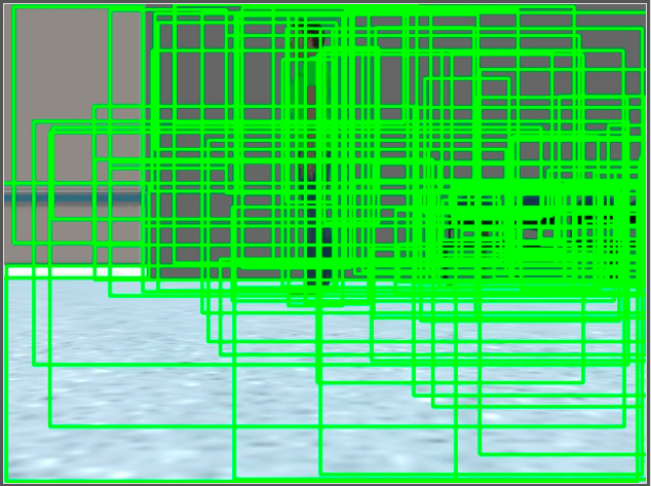
\includegraphics[width=10cm]{imagenes/deteccion-ssd-sin-filtro.png}
  \end{center}
  \caption[Detección mediante SSD sin filtro]{Detección mediante SSD sin filtro}
  \label{fig:deteccion_ssd_sin_filtro}
\end{figure}\

Sin embargo, un modelo de red neuronal genera una puntuación o \textit{score} para cada objeto detectado dependiendo de su entrenamiento, por ejemplo, en una imágen donde puede aparecer una persona y una escultura humana, es probable, que la persona detectada tenga una puntuación de un 90 \% y la escultura un 70 \% debido a su parecido. Está en la labor del programador filtrar por score para desechar los falsos positivos. Para ello, generamos una función que llamaremos \textit{bounding\_boxes\_by\_score(bounding\_boxes, score\_limit)} que filtre aquellos bounding boxes que superen una puntuación límite. Debido a la naturaleza de este modelo neuronal preentrenado, las óptimas detecciones se han comprobado empíricamente que funcionan con una puntuación superior a 0.3 (el rango va de 0 a 1). Aplicando el filtro obtenemos el siguiente resultado (Figura \ref{fig:deteccion_ssd_filtro_score})\\

\begin{figure} [H]
  \begin{center}
    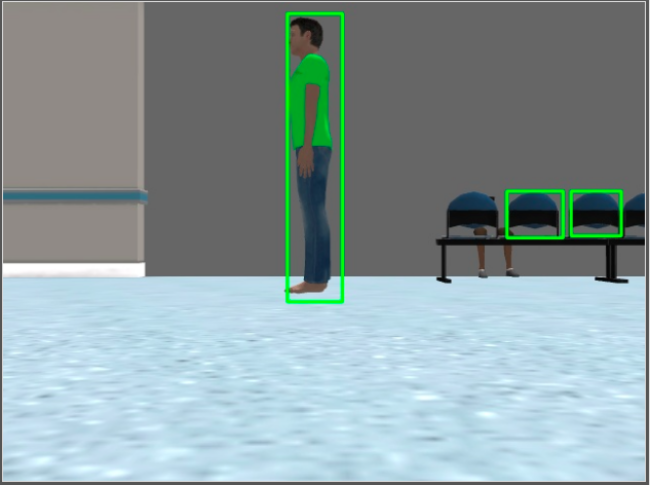
\includegraphics[width=10cm]{imagenes/deteccion-ssd-filtro-score.png}
  \end{center}
  \caption[Detección mediante SSD filtrando el \textbf{Score}]{Detección mediante SSD filtrando el \textbf{Score}}
  \label{fig:deteccion_ssd_filtro_score}
\end{figure}\

Tal y como vemos en la figura \ref{fig:deteccion_ssd_filtro_score}, tras el filtro de puntuación obtenemos una imagen donde hay 3 Bounding Boxes detectados: una persona y 2 sillas. Para quedarnos solo con las personas aplicaremos un \textit{segundo filtro}, en la cual nos fijaremos en la clase del Bounding Box. Recordemos que el objeto Bounding Box tenía un atributo \textit{id} que correspondía a un número entero y un atributo \textit{class\_id} que era la traducción de dicho número a una cadena de texto (ej: 1 - ``person", 2 - ``bicycle"). Crearemos una función llamada \textit{bounding\_boxes\_by\_name(bounding\_boxes, name)} al cual dada una lista de objetos detectados pasaremos como segundo parámetro de entrada el nombre de la clase que queremos filtrar (en este caso ``person"). Aplicando el filtro obtenemos una correcta detección de personas (Figura \ref{fig:deteccion_ssd_filtro_score_class}):\\

\begin{figure} [H]
  \begin{center}
    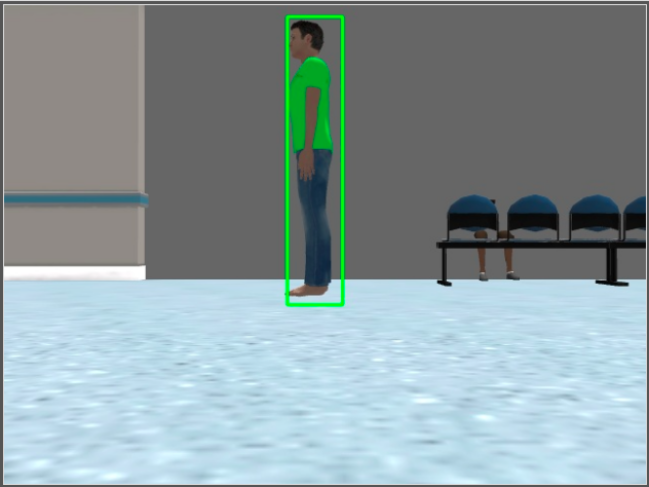
\includegraphics[width=10cm]{imagenes/deteccion-ssd-filtro-score-class.png}
  \end{center}
  \caption[Detección mediante SSD filtrando la puntuación y la clase]{Detección mediante SSD filtrando la puntuación y la clase}
  \label{fig:deteccion_ssd_filtro_score_class}
\end{figure}

Como último filtro y muy recomendable es rechazar aquellas detecciones que no superen un \textit{área} determinado. Con este filtro, evitamos que el robot se confunda con personas que se encuentren a una distancia lejana o con un falso positivo, para ello, crearemos una función llamada \textit{bounding\_boxes\_by\_area(bounding\_boxes, min\_area)} al cual dada una lista de objetos detectados pasaremos como segundo parámetro de entrada el área mínima que debe filtrar.\\

El siguiente paso es crear un \textit{Tracker} de seguimiento. Nuestro tracker se basará en la distancia de los centroides de los Bounding Boxes del fotograma actual con el candidato del fotograma anterior. Recordemos que un Bounding Box tenía otros 4 parámetros más: $x_{min}$ e $y_{min}$ correspondían a las coordenadas (x,y) del extremo superior izquierdo de la caja de detección, y $x_{max}$ e $y_{max}$ correspondían a las coordenadas (x,y) del extremo inferior derecho. Para obtener el centroide aplicaremos la siguiente fórmula:\\
\begin{eqnarray*}
C_x = \frac{x_{min} + x_{max}}{2}\\
C_y = \frac{y_{min} + y_{max}}{2}\\
\end{eqnarray*}

Crearemos una clase llamada \textit{BoundingBoxObject} que tendrá 3 atributos: El Bounding Box correspondiente, su centroide y su área. El área lo obtendremos de la siguiente manera: $A = (x_{max} - x_{min}) (y_{max} - y_{min})$.\\

Posteriormente, creamos una clase llamada \textit{Tracker} que nos proporcionará una capa de abstracción al usar los siguientes métodos que definiremos:

\begin{itemize}
	\item \textbf{setObjective(self, obj)}: Establece el objetivo BoundingBoxObject de seguimiento.
	\item \textbf{getObjective(self)}: Devuelve el objetivo BoundingBoxObject actual de seguimiento.
	\item \textbf{getObjectiveFromSet(self, objlist)}: Dada una lista o conjunto de objetos BoundingBoxObject, devuelve el objetivo candidato que más se acerca al anterior, y lo actualiza. El candidato seleccionado será aquel cuyo centroide esté más cerca del actual, no supere una distancia límite(50) con él, y que la diferencia de área entre el BoundingBoxObject anterior y el actual sea menor a 30000. Para calcular la distancia entre centroides usaremos la \textit{Distancia Euclídea}:
	\begin{equation*}
	d = \sqrt{(C_{x}' - C_{x})^2 + (C_{y}' - C_{y})^2}
	\end{equation*}
\end{itemize}\

En la figura \ref{fig:obtencion_centroide} podemos ver con más detalle en qué se basa esté procedimiento: comparamos cada centroide con el centroide candidato del fotograma anterior y elegiremos aquel que cumpla los requisitos descritos anteriormente.\\

\begin{figure} [H]
  \begin{center}
    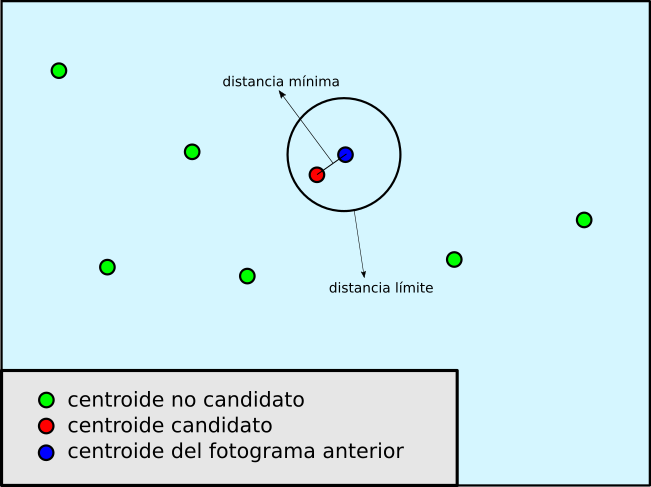
\includegraphics[width=10cm]{imagenes/esquema-tracker.png}
  \end{center}
  \caption[Modo de obtención del centroide candidato]{Modo de obtención del centroide candidato}
  \label{fig:obtencion_centroide}
\end{figure}\

Al principio del programa inicializamos una instancia de tipo Tracker, y, en cada iteración del bucle principal llamamos al método \textit{getObjectiveFromSet(self, objlist)} para obtener un BoundingBoxObject que dibujamos en la imagen de color rojo. El resultado queda de la siguiente manera:\\

\begin{figure} [H]
  \begin{center}
    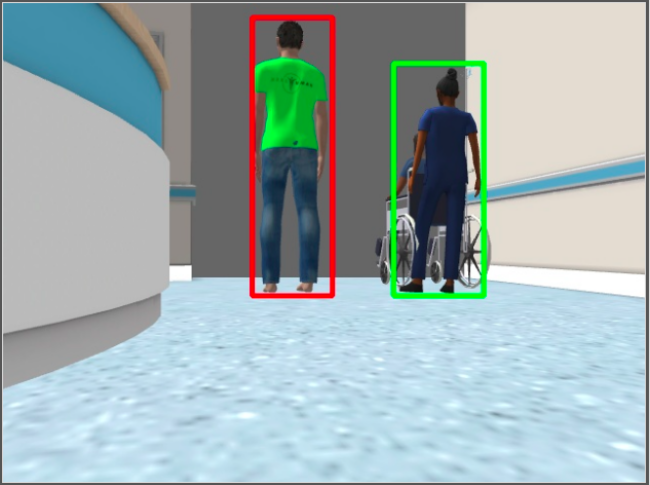
\includegraphics[width=10cm]{imagenes/aplicando-tracker.png}
  \end{center}
  \caption[Usando el Tracker para no perder al objetivo]{Uso del Tracker para no perder al objetivo}
  \label{fig:uso_tracker}
\end{figure}\

Como criterio de selección de la persona a la que seguiremos, deberá cumplir los 3 filtros indicados anteriormente, aparecer en el segundo tercio de la imagen (dividiremos la imagen en 3 y analizaremos la mitad) y ser aquel BoundingBoxObject con un área mayor que el resto.\\


% -- SUBSECCIÓN EVITAR OBSTÁCULOS
% ---------------------------------
\subsection{Algoritmo VFF}
\label{subsec:vff}

Seguir a una persona en un mundo vacío es sencillo, pero cuando el entorno presenta obstáculos, es importante tener ese riesgo en cuenta:\\

\begin{itemize}
	\item ¿Qué ocurre si la persona que seguimos gira por un pasillo a la derecha?. ¿El robot sufriría una colisión con la pared antes de girar?
	\item ¿Qué ocurre si el robot se está acercando a la pata de una mesa? ¿Y si está pasando cerca de otra persona a la que ha descartado en el proceso de Tracking?
\end{itemize}\

El algoritmo de \textit{Campo de Fuerzas Virtuales (VFF)} es el más indicado para esas situaciones. Se basa en la suma vectorial de un vector de atracción y de repulsión originando un vector resultante que indica la nueva dirección de desplazamiento. La suma vectorial estará influenciada por el valor de unos pesos $\alpha$ y $\beta$ aplicados a los vectores de atraccion y repulsión respectivamente, pudiendo de esta manera, dar más valor a uno que otro.\\

El \textit{vector de atracción} será aquel que desde el robot apuntará al objetivo. Al usar una cámara en la que no tenemos en cuenta la profundidad, estableceremos que el módulo del vector será siempre 2 metros. Para obtener el ángulo nos basaremos en el Campo de Visión (FOV) horizontal de la cámara. Al ser una cámara simulada, en su fichero urdf.xacro (tal y como vimos en el capítulo \ref{cap:capitulo4}) indicamos que FOV fuera 1.04 radianes (60 grados). Por lo tanto, 0 grados se corresponderá al centro de la imagen y los extremos a los ángulos -30 y 30. Para conocer el ángulo con el objetivo necesitaremos conocer el ancho de la imagen, y la posición de la coordenada x del centroide. La ecuación es la siguiente:

\begin{equation*}
\alpha = \frac{H_{FOV} \cdot C_{x}}{w} - \frac{H_{FOV}}{2}
\end{equation*}\\

Conociendo el ángulo ($\alpha$) y módulo (m) podremos obtener las componentes x e y del vector de atracción \textit{A}:
\begin{eqnarray*}
A_x = m \cdot sin(\alpha)\\
A_y = m \cdot cos(\alpha)\\
\end{eqnarray*}

El \textbf{vector de repulsión} se calculará a partir de todas las lecturas del láser. Cada obstáculo presente en el rango del láser provocará un vector en sentido contrario cuyo módulo estará influenciado por una constante y será inversamente proporcional a la distancia con el obstáculo (es decir, cuanto más cerca, mayor será el módulo). Sabiendo la constante (K) y la distancia (d) de cada lectura del láser (n lecturas), la ecuación del vector de repulsión (R) es la siguiente:

\begin{eqnarray*}
R_x &=& \sum_{i=1}^n\left(\frac{K}{d_i}\right)^2 \cdot cos(\alpha)\\
R_y &=& \sum_{i=1}^n\left(\frac{-K}{d_i}\right)^2 \cdot sin(\alpha)\\
\end{eqnarray*}

En la ecuación vemos como la componente $R_y$ va en dirección contraria al desplazamiento del robot. La potencia de 2 se aplica para evitar \textbf{mínimos locales}\\

El \textbf{vector final (F) o resultante} lo obtendremos sumando las componentes de los vectores de atracción y repulsión. Ambos multiplicados por dos constantes $\alpha$ y $\beta$ respectivamente. La ecuación queda de esta manera:

\begin{eqnarray*}
F_x &=& \alpha \cdot A_x + \beta \cdot R_x\\
F_y &=& \alpha \cdot A_y + \beta \cdot R_y\\
\end{eqnarray*}

Queda en la labor del programador ajustar empíricamente los parámetros $\alpha$ y $\beta$ dependiendo del comportamiento que desee. Si queremos darle más peso a la repulsión aumentaremos $\beta$ pero en casos extremos podríamos llegar a perder el objetivo. En cambio si queremos darle más peso a la atracción conseguiremos que evité los obstáculos sin perder al objetivo pero si está mal ajustado podríamos colisionar a causa de una escasa repulsión. En la figura \ref{fig:esquema_vff} resumimos el algoritmo VFF de manera gráfica para una mejor comprensión.\\

\begin{figure} [H]
  \begin{center}
    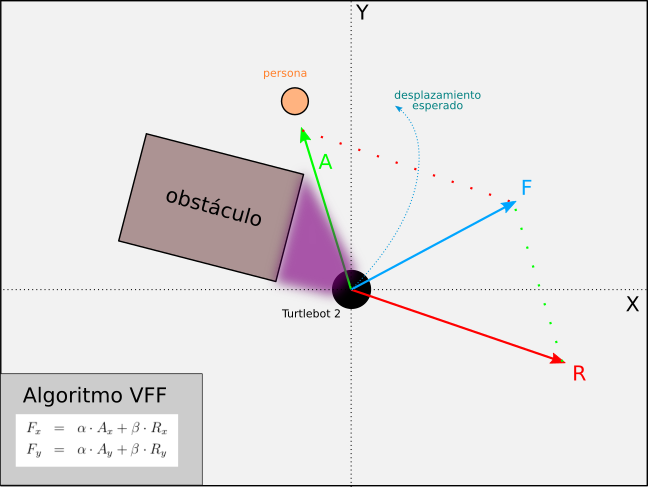
\includegraphics[width=10cm]{imagenes/esquema-vff.png}
  \end{center}
  \caption[Algoritmo VFF]{Algoritmo VFF}
  \label{fig:esquema_vff}
\end{figure}\

En nuestra solución de referencia, aplicaremos solamente la componente $F_x$ como velocidad angular, ya que la velocidad lineal estará \textit{basado en casos} dependiendo de la distancia al objetivo. En el siguiente apartado [\ref{subsec:maquina_estados}] lo explicaremos con más detalle.\\



% -- SUBSECCION MÁQUINA DE ESTADOS
% ----------------------------------
\subsection{Máquina de Estados}
\label{subsec:maquina_estados}

Como último paso de la solución, queda implementar una máquina de estados que le dé al robot la capacidad de tomar distintas acciones dependiendo del estado en el que se encuentre. En nuestro caso, hemos definido 2 estados: Buscar-Persona y Seguir-Persona.\\

El estado \textit{Buscar-Persona} será aquel con el que empecemos la ejecución del programa. Al principio, girará a una velocidad angular determinada mientras aplica los 3 filtros de detección sobre la imagen para detectar personas. Transitará al siguiente estado cuando el robot identifique un candidato a seguir (mayor área del BoundingBoxObject y posicionado en la franja central de la imagen).\\

En el estado \textit{Seguir-Persona} aplicaremos el algoritmo de \textit{Tracking} [\ref{subsec:ml_tracker}] y VFF [\ref{subsec:vff}]. Además, la velocidad lineal cambiará dependiendo de la distancia al objetivo. Para ello crearemos unas condiciones en las que dependiendo del área del Bounding Box aplicaremos una velocidad u otra. Cuanto más pequeño sea el área, más lejos estará nuestro objetivo. Si por algún motivo perdemos a la persona, incrementaremos un contador de fallo y de esta manera, en caso de no detectarla en el siguiente fotograma, nos quedaremos con el mismo valor del centroide candidato. Cuando el contador supere un límite, transitaremos al primer estado: \textit{Buscar-Persona}.\\

El resultado de la solución podemos verla en el siguiente enlace:\\ \textit{\url{https://youtu.be/fDAU465eVxQ}}\\


\section{Solución Sigue-Personas Real}
\label{sec:solucion_sigue_personas_real}

El modo de resolver este problema es idéntico al Sigue-Personas simulado, sin embargo, el entorno sobre el que se mueve el robot, y el rendimiento del ejercicio debido a una distinta carga computacional causada por la ausencia del simulador puede provocar que el comportamiento de la ejecución no sea el esperado.\\

En la \textit{solución} de referencia seguimos los mismos pasos que en la sección [\ref{sec:sigue_personas_simulado}]:\\

\begin{itemize}
	\item Implementación del \textit{Tracker} de seguimiento. Los pasos son los mismos:
	\begin{enumerate}
		\item Localizar a una persona aplicando los filtros de \textit{score} o puntuación, cláse y área.
		\item Aplicaremos el criterio de \textit{selección}: dividir la imagen en 3 secciones y elegir como objetivo la persona más cercana que esté situada en la sección central
		\item Crear una clase Tracker que guarde constantemente y vaya actualizando el objetivo de seguimiento por cada fotograma.
		\item Para no perder al objetivo, en cada fotograma nos quedaremos con el centroide del \textit{Bounding Box} más cercano al centroide candidato del fotograma anterior, mientras no supere un límite de distancia. En caso de no detectar al objetivo, iremos incrementando un contador de fallo.
	\end{enumerate}
	\begin{figure} [H]
		\begin{center}
			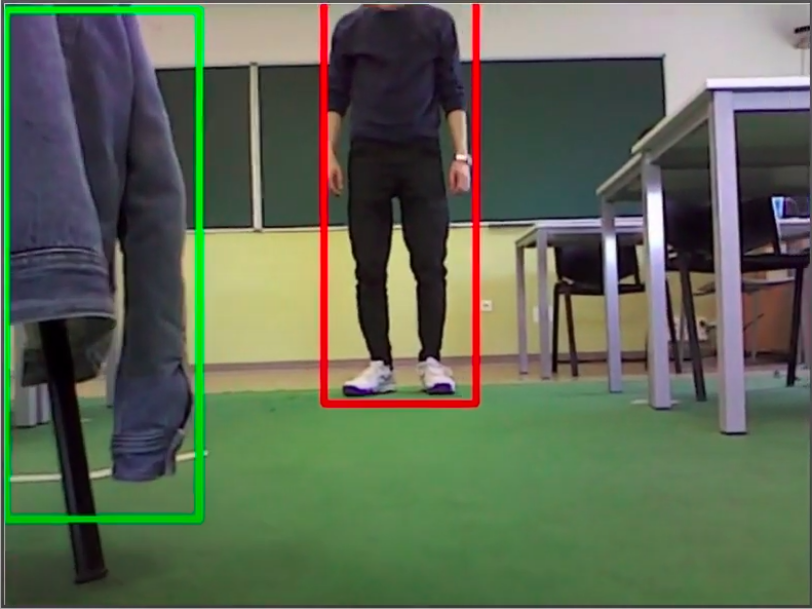
\includegraphics[width=10cm]{imagenes/cap6/tracker.png}
		\end{center}
		\caption[Tracker en el ejercicio Real Follow Person]{Tracker en el ejercicio Real Follow Person}
		\label{fig:tracker_real_follow_person}
	\end{figure}\
	
	\item Implementación del algoritmo VFF. Como la frecuencia de actualización cambia ante la ausencia del simulador, ha sido necesario reajustar los parámetros $\alpha$ y $\beta$ del algoritmo, para equilibrar la relación entre la fuerza de atracción y de repulsión. Es recomendable que el párametro $\alpha$ que multiplica a la fuerza de atracción sea mayor que $\beta$ para no perder al objetivo. Sin embargo, tenemos que tener en cuenta que $\beta$ debe estar correctamente ajustado para esquivar con seguridad y suavidad los obstáculos que se encuentre por su camino. Un buen ajuste de parametros permitirá por ejemplo seguir a una persona a través de un pasillo manteniendo la misma distancia con ambas paredes sin importar la colocación de su objetivo.
	
	\item Máquina de Estados Finitos. Seguimos usando dos estados maestros: Buscar-Persona y Seguir-Persona. La transición del estado Seguir-Persona a Buscar-Persona estaba determinado por el contador de fallo que indiciamos en el proceso de seguimiento del Tracking. El límite del contador dependerá de los fotogramas por segundo. En el ejercicio \textit{Follow Person} simulado, la velocidad de fotogramas era baja por lo tanto el límite era menor, pero en este caso, al haber aumentado la velocidad de refresco, tiene sentido aumentar el límite del contador para que, de esta manera, si perdemos a la persona en un fotograma, podamos seguir guardando el centroide del útlimo \textit{Bounding Box} candidato.
\end{itemize}\

El resultado de la solución podemos verlo en el siguiente enlace:\\
\textit{\url{https://youtu.be/54Jb4KJwyDM}}\\



% -- SECCION VARIANTES
% ----------------------
\section{Variantes de la solución}
\label{sec:variantes_solucion}

La solución mostrada en las secciones [\ref{sec:solucion_sigue_personas_simulado}] y [\ref{sec:solucion_sigue_personas_real}] no es lá unica para abordar el problema. Podemos enfocar el problema Sigue Personas de varias maneras. A continuación indicamos algunas posibles opciones que tuvimos en cuenta antes de llegar a la solución final de referencia:\\

\begin{itemize}
	\item \textbf{Control de velocidad basado en franjas}. En este modelo de seguimiento, dividimos la imagen en franjas y dependiendo de la posición $C_{x}$ del centroide usamos una velocidad angular determinada. A continuación mostramos un ejemplo de implementación
\begin{code}[H]
\begin{lstlisting}
vels = [0.3, 0.2, 0.1, 0, -0.1, -0.2, -0.3]	 # vel > 0 === left turn

width = img.shape[1]
step = width/len(vels)

while True:
	# ...
	cx, cy = centroid
	# ...
	
	HAL.setW(vels[int(cx/step)]) # Angular velocity
\end{lstlisting}
\caption{Ejemplo de control de velocidad basado en franjas}
\label{cod:vel_bar}
\end{code}
	\item \textbf{Velocidad basada en un controlador PID}. Con un controlador PID bien configurado obtendríamos una respuesta rápida y precisa para no perder a la persona. Su algoritmo de seguimiento sería semejante al ejercicio \textit{Follow Line} \footnote{\textbf{Follow Line}: \url{http://jderobot.github.io/RoboticsAcademy/exercises/AutonomousCars/follow_line/}}. Una desventaja de usar un controlador PID es el hecho de verse afectado a causa de una baja velocidad de fotogramas por segundo. Además, tendríamos que tener en cuenta la fuerza repulsiva del láser a la hora de comandar velocidades angulares.
	\item \textbf{Detección de color}. Como solución de escape en caso de tener problemas de alto de rendimiento, pensamos poner al alcance la opción de seguir a la persona dependiendo del color de la camiseta. En el caso del hospital pusimos la camiseta del modelo teleoperado de color verde para facilitar la detección). En un escenario real, la persona podría ponerse alguna camiseta de algún color llamativo para facilitar la detección. Para abordar esa solución, tendríamos que seguir estos pasos:
	\begin{enumerate}
		\item Cambiar el espacio de color de la imagen de RGB a HSV\footnote{\textbf{HSV}: \url{https://es.wikipedia.org/wiki/Modelo_de_color_HSV}}. El espacio HSV (Hue, Saturation, Value) facilita la detección de colores.
		\item Obtener el rango HSV de valores mínimo y máximo del color de la camiseta y crear una máscara que la filtre correctamente.
		\item Siendo $p_{i}$ el valor del pixel (0 o 1) de la máscara y $x_i$ las coordenadas del pixel correspondiente, el centroide lo obtendremos de la siguiente manera (ecuacion obtenida de \cite{centroide_ecuacion}):
		\begin{equation*}
		c = \frac{\sum_{i=1}^n\left(p_i \cdot x_i\right)}{\sum_{i=1}^n\left(p_i\right)}
		\end{equation*}
		\item Una vez obtenido el centroide, aplicar el algoritmo VFF igual que en la solución de referencia.
	\end{enumerate}
\end{itemize}

